\documentclass[a5paper,headsepline,titlepage,12pt,nnormalheadings,DIVcalc,twoside]{scrbook}
\usepackage[a5paper,backref]{hyperref}
%\usepackage{palatino}
\usepackage{graphicx}
\usepackage{wrapfig}
\usepackage[bahasa]{babel}
\usepackage{fancyhdr}
\usepackage{pst-text}
\usepackage{pst-grad}

%\setlength{\voffset}{0.5in}
%\setlength{\oddsidemargin}{28pt}
%\setlength{\evensidemargin}{0pt}
\renewcommand{\footrulewidth}{0.5pt}
\lhead[\fancyplain{}{\thepage}]%
      {\fancyplain{}{\rightmark}}
\rhead[\fancyplain{}{\leftmark}]%
      {\fancyplain{}{\thepage}}
\pagestyle{fancy}
\lfoot[\emph{Misa peringatan \peringatan ~\namaalm}]{}
\rfoot[]{\emph{Misa peringatan \peringatan ~\namaalm}}
\cfoot{}
%\usepackage{landscape}

\setlength{\parindent}{0mm}
\makeatletter
\newcommand{\lagu}[1]{%
  {\parindent \z@ 
    \interlinepenalty\@M \slshape \mdseries \large \textit{#1}\par\nobreak \vskip 10\p@ }}
\newcommand{\keterangan}[1]{%
  {\parindent \z@ 
    \interlinepenalty\@M \slshape \mdseries \textit{#1}\par\nobreak \vskip 10\p@ }}
\makeatother

\newcommand{\BU}[1]{\begin{itemize} \item[U:] #1 \end{itemize}}
\newcommand{\BI}[1]{\begin{itemize} \item[I:] #1 \end{itemize}}
\newcommand{\BIU}[1]{\begin{itemize} \item[I+U:] #1 \end{itemize}}
\newcommand{\BP}[1]{\begin{itemize} \item[P:] #1 \end{itemize}}
\newcommand{\inputlagu}[1]{\begin{textit} \input{#1} \end{textit}}
\newcommand{\namaalm}{Bapak Yohanes Markus Gegono Purwadi}
\newcommand{\namaromo}{Ign Yulianto, OMI}
\newcommand{\peringatan}{1000 hari}
\newcommand{\Peringatan}{Seribu hari}

\begin{document}
\thispagestyle{empty}
%\newsavebox\IBox
%\sbox\IBox{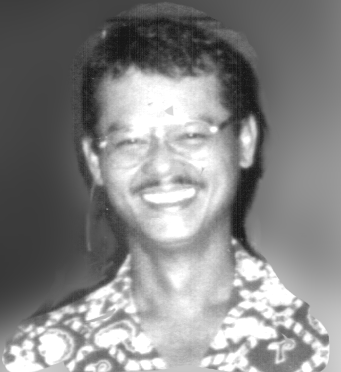
\includegraphics[scale=0.25]{titus.png}}
% set up the picture environment
\psset{unit=1in}
\begin{pspicture}(4in,5in)
% set up the fonts we use
\DeclareFixedFont{\PT}{T1}{ppl}{b}{it}{0.5in}
\DeclareFixedFont{\PTsmall}{T1}{ppl}{b}{it}{0.4in}
\DeclareFixedFont{\PTsmaller}{T1}{ppl}{b}{it}{0.25in}
\DeclareFixedFont{\PTsmallest}{T1}{ppl}{b}{it}{0.2in}
\DeclareFixedFont{\PTtext}{T1}{ppl}{b}{it}{11pt}
\DeclareFixedFont{\Logo}{T1}{pbk}{m}{n}{0.3in}
% place the front cover picture
%\rput[cb](2.3,1.5){\usebox\IBox}
% put the text on the front cover
\rput[cb](2.3,4.5){\PTsmall {EKARISTI}}
\rput[cb](2.3,4.1){\PTsmall {PERINGATAN \MakeUppercase{\Peringatan}}}
\rput[cb](2.3,3.0){\PTsmaller {\namaalm}}
%\rput[cb](2.3,2.6){\PTsmallest(12 Februari 1961 - 04 Maret 2007)}
\rput[cb](2.3,0.4){\PTsmallest {oleh}} 
\rput[cb](2.3,0){\PTsmallest {Rm \namaromo}}
\rput[cb](2.3,-0.4){\PTsmallest {19 Desember 2011}}

%\rput[cb](3,-1){\PTsmallest {\namagereja}} 

\end{pspicture}

\newpage

\begin{center} Romo \namaromo\\
"ALLAH SUMBER SUKACITA SEJATI"\\
MISA KUDUS PERINGATAN \MakeUppercase{\peringatan}\\
\namaalm\\
19 Desember 2011\\
\end{center} 

\section*{RITUS PEMBUKA}

\lagu{Lagu pembuka}

\subsection*{Seruan tobat}

\lagu{Tuhan Kasihanilah Kami}

\subsection*{Doa Pembuka}
\BI{Marilah berdoa\\
	Allah Bapa sumber sukacita, kami telah menerima jaminan kebahagiaan abadi dalam Diri Yesus Kristus Putera-Mu. Kami serahkan hamba-Mu, Bp. Yohanes Markus Gegono Purwadi yang telah Engkau panggil \peringatan ~yang lalu dalam sukacita surgawi. Persatukanlah kami dalam pengharapan akan kebahagiaan kekal di surga, kendati masih harus berjuang di dunia ini. Bantulah kami agar memiliki sukacita sejati dan saling menghibur satu sama lain. Dengan pengantaraan Yesus Kristus PuteraMu Tuhan kami yang bersama dengan Dikau dalam persekutuan Roh Kudus hidup dan berkuasa, Allah sepanjang segala masa.}

\BU{Amin}

\section*{LITURGI SABDA}

\subsection*{Bacaan I}

\BP{\emph{Pembacaan dari Surat pertama Rasul Paulus kepada Jemaat di Korintus (1 Kor 15:16-17,20-22)}

Sebab jika benar orang mati tidak dibangkitkan, maka Kristus juga tidak dibangkitkan.
Dan jika Kristus tidak dibangkitkan, maka sia-sialah kepercayaan kamu dan kamu masih hidup dalam dosamu.

Tetapi yang benar ialah, bahwa Kristus telah dibangkitkan dari antara orang mati, sebagai yang sulung dari orang-orang yang telah meninggal.
Sebab sama seperti maut datang karena satu orang manusia, demikian juga kebangkitan orang mati datang karena satu orang manusia.
Karena sama seperti semua orang mati dalam persekutuan dengan Adam, demikian pula semua orang akan dihidupkan kembali dalam persekutuan dengan Kristus.

}

\BP{Demikianlah Sabda Tuhan}

\BU{Syukur kepada Allah}

\lagu{Lagu Tanggapan/Pengantar}

\subsection*{Bacaan Injil}

\BI{Tuhan sertamu}
\BU{dan sertamu juga}
\BI{Inilah Injil Yesus Kristus menurut Yohanes (17:6-10)}
\BU{Dimuliakanlah Tuhan}

\BI{
Pada suatu ketika Tuhan Yesus bersabda: "Aku telah menyatakan nama-Mu kepada semua orang, yang Engkau berikan kepada-Ku dari dunia. Mereka itu milik-Mu dan Engkau telah memberikan mereka kepada-Ku dan mereka telah menuruti firman-Mu.
Sekarang mereka tahu, bahwa semua yang Engkau berikan kepada-Ku itu berasal dari pada-Mu.
Sebab segala firman yang Engkau sampaikan kepada-Ku telah Kusampaikan kepada mereka dan mereka telah menerimanya. Mereka tahu benar-benar, bahwa Aku datang dari pada-Mu, dan mereka percaya, bahwa Engkaulah yang telah mengutus Aku.

Aku berdoa untuk mereka. Bukan untuk dunia Aku berdoa, tetapi untuk mereka, yang telah Engkau berikan kepada-Ku, sebab mereka adalah milik-Mu
dan segala milik-Ku adalah milik-Mu dan milik-Mu adalah milik-Ku, dan Aku telah dipermuliakan di dalam mereka."
}

\subsection*{Homili}
\subsection*{Doa Umat}

\BI{Saudara-saudari, kehadiran kita bersama ini mengungkapkan iman kita akan Allah sumber sukacita sejati. Marilah dengan rendah hati kita ungkapkan doa dan permohonan kita kepada Bapa:}

\BP{Ya Bapa, kedatangan Yesus Kristus di tengah-tengah kami menghadirkan tahun rahmat Tuhan kepada manusia. Semoga peringatan \Peringatan ~meninggalnya \namaalm inipun meng
hadirkan tahun rahmat bagi kita semua yang mengikuti Perayaan Ekaristi ini.

Kami mohon \dots}

\BU{Kabulkanlah doa kami, ya Tuhan.}

\BP{Bagi keselamatan jiwa \namaalm yang telah berpulang: 

Semoga ia diberi tempat yang layak di dalam Kerajaan Surga.

Kami mohon \dots}

\BU{Kabulkanlah doa kami, ya Tuhan.}

\BP{Bagi keluarga yang ditinggalkan: Semoga mereka selalu tabah menerima peristiwa hidupnya yang terasa menekan dan menyandarkan diri sepenuhnya pada belas kasih Tuhan.

Kami mohon \dots}

\BU{Kabulkanlah doa kami, ya Tuhan.}

\BP{Bagi semua orang yang meninggal: Semoga karena kerahiman Tuhan mereka diijinkan memandang kemuliaan wajah Allah.

Kami mohon \dots}

\BP{Bagi kita sendiri: Semoga kita selalu terbuka hati untuk menolong sesama kita yang mengalami kesulitan dalam hidupnya.

Kami mohon \dots}

\BU{Kabulkanlah doa kami, ya Tuhan.}

\BI{Bapa kasihMu tiada batas, kesabaranMu begitu besar. Semoga dalam pengharapan iman yang benar, kami senantiasa dalam limpahan rahmatMu, dengan pengantaraan Kristus Tuhan kami.}

\section*{LITURGI EKARISTI}

\lagu{Lagu Persembahan}
\subsection*{Persiapan Persembahan}

\BI{Terpujilah Engkau ya Tuhan, Allah semesta alam, sebab dari kemurahanMu, kami menerima roti yang kami siapkan ini. Inilah hasil dari bumi dan dari usaha manusia yang bagi kami akan menjadi roti kehidupan.}

\BU{Terpujilah Allah selama-lamanya}

\BI{Terpujilah Engkau ya Tuhan, Allah semesta alam, sebab dari kemurahanMu, kami menerima anggur yang kami siapkan ini. Inilah hasil dari pohon anggur dan dari usaha manusia yang bagi kami akan menjadi minuman rohani.}

\BU{Terpujilah Allah selama-lamanya}

\BI{Berdoalah saudara-saudari, supaya persembahanku dan persembahanmu berkenan pada Allah Bapa yang Mahakuasa.}

\BU{Semoga persembahan ini diterima demi kemuliaan Tuhan dan keselamatan kita serta seluruh umat Allah yang kudus.}

\subsection*{Doa Persiapan Persembahan}

\BI{Allah Bapa sumber kekudusan, terimalah bahan persembahan roti dan anggur yang kami hunjukkan untuk keselamatan hamaMu \namaalm. Perkenankanlah dia memasuki rumahMu di surga, dan anugerahkan kami semua ketekunan dalam penghapran. Demi Kristus Tuhan dan pengantara kami.}

\BU{Amin.}


\subsection*{Doa Syukur Agung}

\lagu{Kudus}

\lagu{Anak Domba Allah}

\subsection*{Ajakan menyambut komuni}

\BI{Saudara-saudari terkasih, Tuhan Yesus bersabda; "Datanglah kepadaKu, kalian yang telah memikul beban berat, maka Aku akan memberikan rasa lega kepadamu." Beban dosa kitapun akan dihapus. Maka berbahagialah kita yang diundang ke perjamuan Tuhan.}

\BU{Ya Tuhan, saya tidak pantas Tuhan datang pada saya, tetapi bersabdalah saja, maka saya akan sembuh.}

\lagu{Lagu Komuni}

\subsection*{Doa sesudah komuni}

\BI{Marilah berdoa,

Allah Bapa sumber kehidupan, kami telah Engkau segarkan dengan santapan kehidupan, Tubuh dan Darah Yesus PutraMu. KehadiranNya memberi keteguhan bagi hidup kami sehari-haru dalam berusaha memenuhi kehendakMu melalui pelayanan da  pekerjaan kami. Semoga hambaMu \namaalm yang telah \Peringatan ~menghadapMu kini berbahagia bersamaMu dan persatukanlah kami kelak dengannya serta para kudus di surga. Dengan perantaraan Kristus Tuhan kami,}

\BU{Amin.}

\section*{RITUS PENUTUP}

\keterangan{Pengumuman dan ucapan terima kasih dari wakil keluarga.}

\subsection*{Berkat Penutup}

\BI{Saudara-saudari yang terkasih, marilah kita mengakhiri perayaan ekaristi dan doa kita untuk \namaalm, dengan mohon berkat Tuhan.}

\BI{Tuhan sertamu}

\BU{Dan sertamu juga}

\BI{Semoga saudara-saudari sekalian yang hadir di sini, dilindungi dan dibimbing oleh berkat Allah yang Mahakuasa Bapa, Putera, dan Roh Kudus}

\BU{Amin.}

\BI{Saudara sekalian, dengan ini perayaan ekaristi dan doa arwah \namaalm sdah selesai}

\BU{Syukur kepada Allah}

\BI{Marilah kita pergi, kita diutus untuk mewartakan damai Tuhan}

\BU{Amin.}

\lagu{Lagu penutup}

\begin{center}
TERIMA KASIH ATAS DUKUNGAN DOA DARI\\
BAPAK, IBU, DAN SAUDARA\\
SEMOGA KEBAIKAN BAPAK, IBU, DAN SAUDARA\\
TUHAN BERKENAN MEMBERKATI
\end{center}
\end{document}
